\documentclass[presentation, 10pt]{beamer}
\usepackage[utf8]{inputenc}
\usepackage{graphicx}
\usepackage{amsmath}
\usepackage{amssymb}
\usepackage{mathtools}
\mathtoolsset{showonlyrefs}
\usetheme{simple}
\usepackage{array}
\usepackage{textcomp}
\newcommand{\textapprox}{\raisebox{0.5ex}{\texttildelow}}
\usepackage{outlines}
\usepackage{multimedia}
\usepackage{bm}

\setbeamertemplate{bibliography item}{\insertbiblabel}

\author{Scott Trinkle}
\date{February 20, 2018}
\title{Update on x-ray / diffusion-MR comparison metrics}

\begin{document}

\frame{\titlepage}

\begin{frame}{Outline}

  \begin{outline}
    \1 Comparing tractography results
    \2 Metrics from ISBI Conference ``3D VoTEM Data Challenge'' and references

    \1 Generating MR-like orientation metrics from ground truth
    \2 Structure tensor analysis
  \end{outline}

\end{frame}

\begin{frame}
  \centering
  \Large Comparing tractography results
\end{frame}

\begin{frame}{ISBI Conference Challenge}

  \begin{outline}
    \1 Three datasets
    \2 ``Anisotropic diffusion phantom''
    \2 MRI and BDA histological tracer injections from same squirrel monkey brain
    \2 MRI from Rhesus Macaque monkey compared to ground truth histological atlas
    \1 Three primary evaluation metrics
    \1 All analysis code will be released at the end of the challenge (submissions due early March, conference in early April)
  \end{outline}
\end{frame}


\begin{frame}{ISBI Conference Challenge - Metrics}
  
\begin{outline}
  \1 ``(1) \textbf{A voxel-wise bundle overlap measure} \cite{ning}. The proportion of voxels within the ground truth volume that are traversed by tractography streamlines. This value describes how well the submitted tractography algorithm is able to recover the volume of the true white matter bundle.''
  
  \1 ``(2) \textbf{A voxel-wise bundle overreach measure} \cite{ning}. The fraction of voxels containing a tractography streamline outside the volume of the gold standard bundle divided by the total number of voxels in the gold standard bundle. This value describes the extent that tractography extends beyond the valid white matter bundles.''
\end{outline}

\end{frame}


\begin{frame}{Ning et al 2015}
  \begin{outline}
    \1 Sparse reconstruction challenge for diffusion MRI
    \2 Comparing 16 reconstruction methods using sparse measurements of a physical phantom
    \2 Gold standard was another MRI dataset with denser measurements

    \1 Normalized mean square error

  
    \begin{equation}
      \text{NMSE} = \frac{1}{|\Omega|} \sum_{x \in \Omega} \frac{||\hat{\bm{s}}_{\bm{x}} - \bm{s}_{\bm{x},\text{gold}}||^2}{||\bm{s}_{\bm{x},\text{gold}}||^2}
    \end{equation}

    \2 $\Omega$ denotes the set of voxel locations, $|\Omega|$ is the total number of voxels, $\hat{\bm{s}}_{\bm{x}}$ is the reconstructed signal vector at location $\bm{x}$ and $\bm{s}_{\bm{x},\text{gold}}$ is the gold-standard signal.\newline

    \1 Estimated angle
    \2 Should have an estimate for the number of crossing fiber bundles by counting peaks in estimated Orientation Distribution Function
    \2 Find matching voxels with multiple peaks and compare estimated angle
    \2 Can also evaluate percentage of false peaks

  \end{outline}

\end{frame}



\begin{frame}{ISBI Conference Challenge - Metrics}

  \begin{outline}
    \1 ``(3) \textbf{A region-of-interest based sensitivity and specificity score} \cite{thomas}. These values will be calculated based on the presence or absence of tractography and tracer tracts on a larger spatial scale (10’s to 100’s of voxels)''
  \end{outline}
  
\end{frame}


\begin{frame}{Thomas et al 2014}

  \begin{outline}
    \1 Comparing different tractography algorithms, using ``known axonal projections from previous tracer studies in the macaque''
    \2 Registered ROI to previously published atlas with different animals
    \1 ROC analysis
    \2 Looking at voxel-wise sensitivity and specificity within a 2D ROI
    \3 ROI from various regions, gray matter vs. white matter, etc.
    \2 Used to evaluate different algorithms and parameters
    \2 Also used to evaluate optimal thresholding for probabilistic tractography algorithms
  \end{outline}

  \centering
  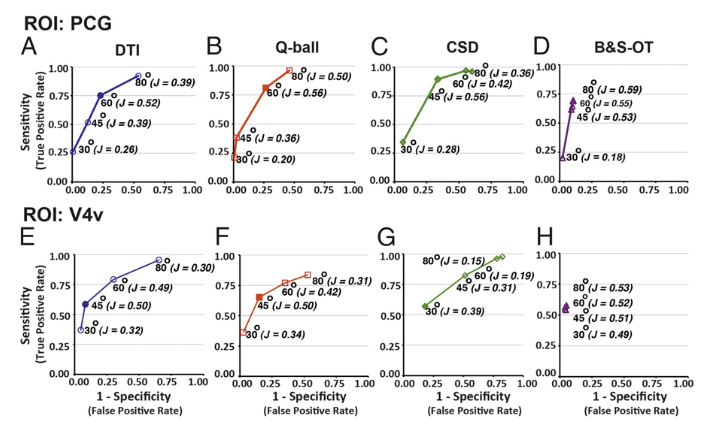
\includegraphics[width=0.5\linewidth]{figs/thomas_roc}
  
\end{frame}

\begin{frame}{Thomas et al}

  \begin{outline}
    \1 ``Despite the exceptional quality of the DWI data, \textbf{none of the methods demonstrated high anatomical accuracy}. The methods that showed the highest sensitivity showed the lowest specificity, and vice versa. Additionally, anatomical accuracy was highly dependent upon parameters of the tractography algorithm, with different optimal values for mapping different pathways.''
  \end{outline}
  
\end{frame}

\begin{frame}{ISBI Conference Challenge - Secondary metrics}

  \begin{outline}
    \1 Hausdorff distance
    \2 From Wikipedia... ``the greatest of all the distances from a point in one set to the closest point in the other set.''
    \1 Correlation of probabilistic score and ground-truth fiber density for probabilistic tractography algorithms. 
  \end{outline}

\end{frame}



\begin{frame}
  \centering
  \Large Generating MR-like orientation metrics from ground truth\newline

  Structure tensor analysis
\end{frame}


\begin{frame}{Budde 2012/13 \cite{budde2012, budde2013}}
  \begin{outline}
    \1 Construct structure tensor from ground truth (histology sections) partial derivative images $f_x$, $f_y$. 

    \begin{equation}
      J = \begin{bmatrix}
        f_x^2 & f_x f_y \\
        f_x f_y & f_y^2
      \end{bmatrix} \times w(x,y)
    \end{equation}

    \2 $w$ is a Gaussian convolution kernel of width $\sigma$.

    \1 Primary orientation (corresponding to largest eigenvector of tensor)

    \begin{equation}
      \theta = \frac{1}{2}\text{arctan}\left(2\frac{f_x f_y}{f_y^2 - f_x^2}\right)
    \end{equation}

    \1 Anisotropy index
    
    \begin{equation}
      \text{AI} = \frac{\lambda_1 - \lambda_2}{\lambda_1 + \lambda_2}
    \end{equation}

    \2 $\lambda_1$ and $\lambda_2$ are the largest and smallest eigenvalues of $J$, respectively.
    
  \end{outline}
\end{frame}

  \begin{frame}{Budde 2012/13 \cite{budde2012, budde2013}}
    \centering
    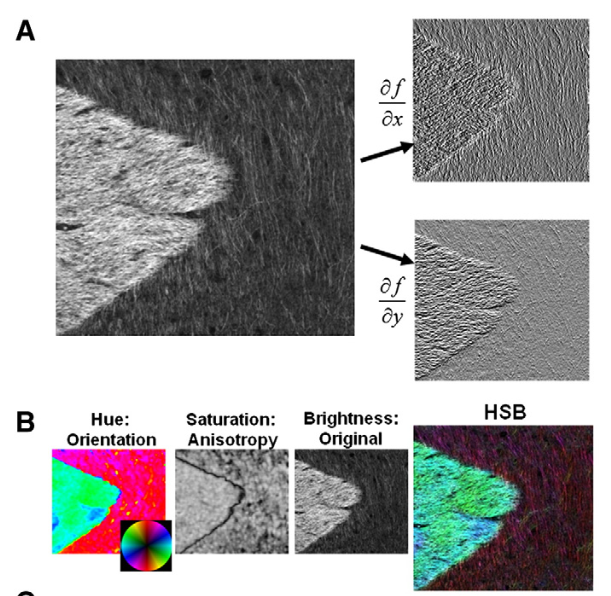
\includegraphics[width=0.9\textheight]{figs/budde_method_1}
  \end{frame}
      
\begin{frame}{Budde 2012/13 \cite{budde2012, budde2013}}
  \begin{outline}
    \1 Downsample histology pixels to MRI dimensions
    \1 Compute Fiber Orientation Distributions (FODs) within downsampled voxel
    \2 Histogram of pixel primary orientations, $\theta$
    \2 Fit to either Gaussian or ``von Mises'' distribution:

    \begin{equation}
      f(\theta|\mu, \kappa) = \frac{e^{\kappa\text{cos}(\theta-\mu)}}{2\pi I_0(\kappa)}
    \end{equation}

    \2 $\kappa$ is concentration ($1 / \kappa$ is analogous to variance), and $\mu$ is center.
    \2 To identify crossing fibers, fit to two-term von Mises distribution, and measure angular difference between $\mu_1$ and $\mu_2$
    \3 Or compare the improvement in adjusted-R$^2$ between single- and double-term  models.
    \1 Compare with MRI with Pearson's correlation within ROI

  \end{outline}
\end{frame}

  \begin{frame}{Budde 2012/13 \cite{budde2012, budde2013}}
    \centering
    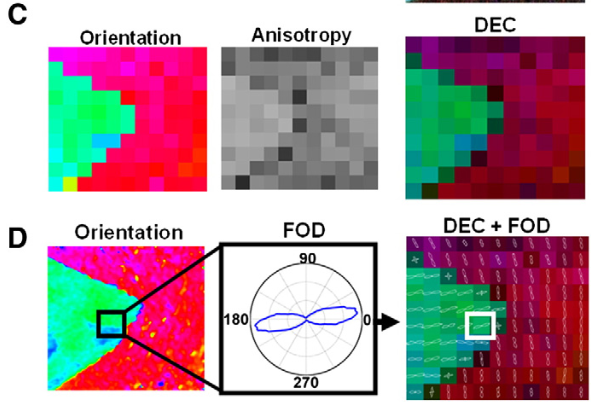
\includegraphics[height=0.9\textheight]{figs/budde_method_2}
  \end{frame}
      

  \begin{frame}{And more!}
    \begin{outline}
      \1 Papers using Budde's structural tensor analysis for diffusion MR validation have used:\newline
      \2 Histology in human samples (and rat, mouse, monkeys, etc.)
      \3 Brain and \textit{in utero}
      \2 Confocal light microscopy
      \3 Extended to 3D
      \2 X-ray microCT
      \3 For fiber orientation in textiles

      \1 Other methods:
      \2 2D/3D Fourier analysis
      \3 Electron Microscopy
      \3 Histology
      \2 Polarized light microscopy
      \2 Serial optical coherence scanning

      \1 Some papers expand FODs in terms of spherical harmonics
    \end{outline}
  \end{frame}

\begin{frame}{References}
  \bibliographystyle{ieeetr}
  \bibliography{comparison_metrics_bib}
\end{frame}

\end{document}
